%%%%%%%%%%%%%%%%%%%%%%%%%%%%%%%%%%%%%%%%%
% Thin Sectioned Essay
% LaTeX Template
% Version 1.0 (3/8/13)
%
% This template has been downloaded from:
% http://www.LaTeXTemplates.com
%
% Original Author:
% Nicolas Diaz (nsdiaz@uc.cl) with extensive modifications by:
% Vel (vel@latextemplates.com)
%
% License:
% CC BY-NC-SA 3.0 (http://creativecommons.org/licenses/by-nc-sa/3.0/)
%
%%%%%%%%%%%%%%%%%%%%%%%%%%%%%%%%%%%%%%%%%

%----------------------------------------------------------------------------------------
%	PACKAGES AND OTHER DOCUMENT CONFIGURATIONS
%----------------------------------------------------------------------------------------

\documentclass[11pt]{article} % Font size (can be 10pt, 11pt or 12pt) and paper size (remove a4paper for US letter paper)

\usepackage[protrusion=true,expansion=true]{microtype} % Better typography
\usepackage{graphicx} % Required for including pictures
\usepackage{wrapfig} % Allows in-line images

\usepackage{mathpazo} % Use the Palatino font
\usepackage[T1]{fontenc} % Required for accented characters
\usepackage[utf8x]{inputenc} % Enecoding used in the document
\usepackage[spanish]{babel}
\linespread{1.05} % Change line spacing here, Palatino benefits from a slight increase by default

\makeatletter
\renewcommand\@biblabel[1]{\textbf{#1.}} % Change the square brackets for each bibliography item from '[1]' to '1.'
\renewcommand{\@listI}{\itemsep=0pt} % Reduce the space between items in the itemize and enumerate environments and the bibliography

\renewcommand{\maketitle}{ % Customize the title - do not edit title and author name here, see the TITLE block below
\begin{flushright} % Right align
{\LARGE\@title} % Increase the font size of the title

\vspace{50pt} % Some vertical space between the title and author name

{\large\@author} % Author name
\\\@date % Date

\vspace{40pt} % Some vertical space between the author block and abstract
\end{flushright}
}

%----------------------------------------------------------------------------------------
%	TITLE
%----------------------------------------------------------------------------------------

\title{\textbf{Solución numerica de ecuaciones diferenciales parciales parabólicas por el método de Crank-Nicolson.}\\ % Title
%Focused and Deliciously Witty Subtitle} % Subtitle
}
\author{\textsc{Roberto Largo Taborda, Duban Arley Medina Eusse} % Author
\\{\textit{Universidad Nacional de Colombia}}} % Institution

\date{\today} % Date

%----------------------------------------------------------------------------------------

\begin{document}

\maketitle % Print the title section

%----------------------------------------------------------------------------------------
%	ABSTRACT AND KEYWORDS
%----------------------------------------------------------------------------------------

\renewcommand{\abstractname}{Resumen} % Uncomment to change the name of the abstract to something else

\begin{abstract}
Las ecuaciones diferenciales parabólicas pueden ser solucionadas computacionalmente mediante dos métodos ampliamente conocidos como lo son el de las diferencias hacia atrás y hacia adelante. El método de diferencias hacia adelante de carácter explicito presenta inestabilidad bajo ciertas condiciones, mientras que el método de las diferencias hacia atrás es de carácter implícito por lo cual es estable, pero con el defecto de que a pesar de que su error de truncación espacial es de orden dos su error de truncación temporal es de orden uno, por lo anterior se hace necesario el estudio de un método que corrija dichos percances, en el documento se estudia como surge el método y su implementación computacional.
\end{abstract}

\hspace*{3,6mm}\textit{Keywords:} lorem , ipsum , dolor , sit amet , lectus % Keywords

\vspace{30pt} % Some vertical space between the abstract and first section

%----------------------------------------------------------------------------------------
%	ESSAY BODY
%----------------------------------------------------------------------------------------

\section*{Introduction}

El método de diferencias hacia adelante es de carácter totalmente explícito, pero con el problema de que sólo para ciertos valores de $\lambda =\frac{\alpha ^2 k}{h^2}$, mas precisamente para $\lambda < \frac{1}{2}$ presenta un comportamiento estable en los cálculos. La primera solución ha sido reemplazarlo por el método de diferencias hacia atrás que no tiene ningún problema de estabilidad, aunque a cambio era un método implícito, precisando de la resolución de un sistema lineal para cada avance del tiempo.

Pero ambos llevaban asociados un orden de truncación del tipo $O(h2) + O(k)$, o sea orden 1 en el tiempo, lo que suele ser poco en los casos prácticos en los que una precisión adecuada obliga a distanciar muy poco los nodos de t, o sea a tomar k muy pequeño. Existe un método que, con la dificultad de ser implícito, no tiene problemas de estabilidad y además posee un orden de truncación $O(h2) + O(k2)$, permitiendo entonces disminuciones menos importantes del paso k manteniendo una buena precisión de los resultados, Este es el denominado método de Crank-Nicolson.

%------------------------------------------------

\section*{Desarollo matemático}

Cras gravida, est vel interdum euismod, tortor mi lobortis mi, quis adipiscing elit lacus ut orci. Phasellus nec fringilla nisi, ut vestibulum neque. Aenean non risus eu nunc accumsan condimentum at sed ipsum.
\begin{wrapfigure}{l}{0.4\textwidth} % Inline image example
\begin{center}
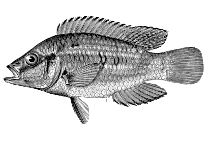
\includegraphics[width=0.38\textwidth]{fish.png}
\end{center}
\caption{Fish}
\end{wrapfigure}
Aliquam fringilla non diam sed varius. Suspendisse tellus felis, hendrerit non bibendum ut, adipiscing vitae diam. Lorem ipsum dolor sit amet, consectetur adipiscing elit. Nulla lobortis purus eget nisl scelerisque, commodo rhoncus lacus porta. Vestibulum vitae turpis tincidunt, varius dolor in, dictum lectus. Aenean ac ornare augue, ac facilisis purus. Sed leo lorem, molestie sit amet fermentum id, suscipit ut sem. Vestibulum orci arcu, vehicula sed tortor id, ornare dapibus lorem. Praesent aliquet iaculis lacus nec fermentum. Morbi eleifend blandit dolor, pharetra hendrerit neque ornare vel. Nulla ornare, nisl eget imperdiet ornare, libero enim interdum mi, ut lobortis quam velit bibendum nibh.

Morbi tempor congue porta. Proin semper, leo vitae faucibus dictum, metus mauris lacinia lorem, ac congue leo felis eu turpis. Sed nec nunc pellentesque, gravida eros at, porttitor ipsum. Praesent consequat urna a lacus lobortis ultrices eget ac metus. In tempus hendrerit rhoncus. Mauris dignissim turpis id sollicitudin lacinia. Praesent libero tellus, fringilla nec ullamcorper at, ultrices id nulla. Phasellus placerat a tellus a malesuada.

%------------------------------------------------

\section*{Algoritmo}

Fusce in nibh augue. Cum sociis natoque penatibus et magnis dis parturient montes, nascetur ridiculus mus. In dictum accumsan sapien, ut hendrerit nisi. Phasellus ut nulla mauris. Phasellus sagittis nec odio sed posuere. Vestibulum porttitor dolor quis suscipit bibendum. Mauris risus lectus, cursus vitae hendrerit posuere, congue ac est. Suspendisse commodo eu eros non cursus. Mauris ultrices venenatis dolor, sed aliquet odio tempor pellentesque. Duis ultricies, mauris id lobortis vulputate, tellus turpis eleifend elit, in gravida leo tortor ultricies est. Maecenas vitae ipsum at dui sodales condimentum a quis dui. Nam mi sapien, lobortis ac blandit eget, dignissim quis nunc.

\begin{enumerate}
\item First numbered list item
\item Second numbered list item
\end{enumerate}

Donec luctus tincidunt mauris, non ultrices ligula aliquam id. Sed varius, magna a faucibus congue, arcu tellus pellentesque nisl, vel laoreet magna eros et magna. Vivamus lobortis elit eu dignissim ultrices. Fusce erat nulla, ornare at dolor quis, rhoncus venenatis velit. Donec sed elit mi. Sed semper tellus a convallis viverra. Maecenas mi lorem, placerat sit amet sem quis, adipiscing tincidunt turpis. Cras a urna et tellus dictum eleifend. Fusce dignissim lectus risus, in bibendum tortor lacinia interdum.

%----------------------------------------------------------------------------------------
%	BIBLIOGRAPHY
%----------------------------------------------------------------------------------------

\bibliographystyle{unsrt}

\bibliography{sample}

%----------------------------------------------------------------------------------------

\end{document}